\documentclass[conference, DIV=14]{IEEEtran}

% Sammlung
\pagestyle{plain}

% Eingabecodierung
\usepackage[utf8]{inputenc}

% Sprachraum
\usepackage[ngerman]{babel}

% Schriftcodierung Europäische Zeichen
\usepackage[T1]{fontenc}

% Schrifteinstellungen
% Vektorschrift
\usepackage{lmodern}
% Serifenlose Schrift 
\renewcommand{\familydefault}{\sfdefault}
% Mathe-Schrift ohne Serifen 
\usepackage{sansmath}
% aktiviert serifenlose Matheschrift  	
\sansmath
% harmonische Typenverteilung 							
\usepackage{microtype}	

% Code einbinden
\usepackage{listings}
\usepackage{minted}

% Literatur einbinden
\usepackage[babel, german=quotes]{csquotes}
\usepackage[
backend=biber,
style=numeric-comp,
block=ragged,			
sorting=none,			
]{biblatex}
\addbibresource{ref_liste.bib}


% Pie Chart
% https://tex.stackexchange.com/questions/500362/using-pgf-pie-to-draw-pie-charts-without-labels-on-the-slices-but-still-able-to
\usepackage{pgf-pie}
\usepackage{etoolbox}
\newtoggle{showpct}
\makeatletter
\patchcmd{\pgfpie@slice}%
{\pgfpie@scalefont{#3}\pgfpie@numbertext{#3}}%
{\iftoggle{showpct}{\pgfpie@scalefont{#3}\pgfpie@numbertext{#3}}{}}%
{}{}
\makeatother

% Mathemodus
\usepackage{amsmath,amssymb}
\usepackage{mathtools}

% Bilder einbinden
\usepackage{graphicx}
\graphicspath{{images/}}

% Grafiken zeichen
\usepackage{tikz}
\usetikzlibrary{calc,arrows,positioning} 
\usepackage{pgfplots}
\pgfplotsset{compat=1.7}

% Zum automatischen und manuellen Erstellung von dynamischen Querverweisen in Dokumenten
\usepackage{hyperref}
\hypersetup{
    colorlinks,
    citecolor=black,
    filecolor=black,
    linkcolor=black,
    urlcolor=black
}

% Tabellen
\usepackage{tabularx}
\usepackage{diagbox}

% Lorem Ipsum
\usepackage{lipsum}

% Eigener enumerate Style
\usepackage{enumerate}

\begin{document}
\title{Löst das Chainweb das Blockchaintrilemma?\\}
\author{\IEEEauthorblockN{Author}
\IEEEauthorblockA{\textit{Semester} \\
\textit{Institution}\\
\textit{Jahr}\\
Ort, Land \\
Kontakt}
}

\maketitle
\begin{abstract}
    Das  Chainweb  möchte  das  Blockchaintrilemma  gelöst  haben.  Dieses besagt,  dass  eine  Blockchain  nur  zwei  dreier  wichtiger  Eigenschaften vereinen kann: Dezentralität, Sicherheit und Skalierbarkeit. Dank  beliebig vieler,  unabhängiger  Ketten  kann  das  Chainweb  effektiver als bisherige  Proof of Work  Blockchains  arbeiten. In dieser Arbeit wird das Chainweb hinsichtlich des Blockchaintrilemmas bewertet und mit anderen Proof of Work Blockchains vergleichen. Es wird dargestellt, wie eine POW-Blockchain auf Layer 1 skalieren kann und erläutert, wie die Sicherheit der Blockchain davon profitiert. Der Punkt der Dezentralität wird untersucht und gezeigt, dass ein Akteur zu viel Rechenleistung im Netzwerk besitzt. \\
\end{abstract}

\begin{IEEEkeywords}
	Blockchain, Chainweb, Blockchaintrilemma, Proof of Work
\end{IEEEkeywords} 
\section{Einleitung}
Blockchaintechnologien ermöglichen es, Vermögen dezentral zu verwalten oder zu versenden. Zusätzlich schafft sie Transparenz, denn jede Transaktion ist öffentlich einsehbar. Über die letzten Jahre haben sich durch mehr Nutzer neue Herausforderungen an die junge Technologie gestellt. Eine Blockchain kann nicht beliebig viele Transaktionen gleichzeitig verarbeiten, denn jeder Block ist auf eine bestimmte Größe limitiert. Mit steigendem Transaktionsaufkommen und gleich bleibendem Angebot an vorhandenem Platz in jedem neuen Block steigt schlussendlich der Preis pro Transaktion. Um das Problem zu lösen, wurden neue Technologien entwickelt: Diese reichen von anderen Konsensfindungsverfahren (Proof of Stake $POS$, delegiertes  Proof-of-Stake $dPOS$) bis hin zu Layer 2 Lösungen oder Quantentechnologie. \cite{BundesamtfurSicherheitinderInformationstechnik.2019}
\\
In dieser Arbeit wird die neue Blockchaintechnologie des Chainwebs betrachtet und bewertet. Es wird die Funktionsweise untersucht und sodann experimentell gezeigt, wie das Chainweb eine Proof of Work Blockchain skaliert. Hierbei steht der Aspekt der Sicherheit eine wesentliche Rolle. 
\section{Blockchain am Beispiel von Bitcoin}
Im Jahr 1991 haben Stuart Haber und W. Scott Stornetta mit ihrer Veröffentlichung \textit{How to Time-Stamp a Digital Document} die Grundlage für uns heute bekannte Blockchains gelegt. Durch Errechnen des Hashwertes eines Dokuments kann auch zu einem späteren Zeitpunkt belegt werden, dass ein Dokument nachträglich nicht verändert wurde. \cite{Haber.1991} 
\\
Darauf aufbauend wurde 2008 das Bitcoin Core Protokoll vorgestellt. Die grundlegende Idee ist es, Anwendern die Möglichkeit zu geben, Transaktionen ohne eine zentrale Institution abzuwickeln. Dazu führt jeder Teilnehmer eine eigene Historie über alle Transaktionen des Netzwerks. Sobald ein neuer Block generiert wurde, wird dieser an alle Teilnehmer des Netzwerks gesendet und in die Kette eingereiht. Dieses Kapitel beschreibt die Funktionsweise einer Proof of Work Blockchain am Beispiel von Bitcoin.

\subsection{Senden von Transaktionen}
Alle Anwender besitzen jeweils einen öffentlichen und einen privaten Schlüssel. Um eine Transaktion von einer Adresse senden zu können, muss der Sender sich mittels des privaten Schlüssels authentifizieren. Dazu signiert er die Transaktion, dargestellt in Formel \eqref{eq:signTransaction}. Es sei $s$ der private Schlüssel, $p$ der öffentliche Schlüssel und $t$ die zu signierende Transaktion.

\begin{equation}
sign(t, s) = Signatur
\label{eq:signTransaction}
\end{equation}

Die Transaktion wird zusammen mit der entstehenden Signatur an alle Teilnehmer des Netzwerks gesendet. Um zu bestätigen, dass einzig der Besitzer des privaten Schlüssels die Transaktion senden konnte, wird  die Korrektheit mittels Formel \eqref{eq:verifyTransaction} bestätigt.

\begin{equation}
verify(t, Signatur, p) = True/False
\label{eq:verifyTransaction}
\end{equation}

Das dezentrale Netzwerk kann so sicher sein, dass der zum öffentlichen Schlüssel passende private Schlüssel die Transaktion signiert hat.

Alice möchte nun 1 BTC an Bob senden. Sie signiert die Transaktion und sendet die entstehende Signatur zusammen mit ihrem öffentlichen Schlüssel und der auszuführenden Transaktion an alle Teilnehmer des Netzwerks. Um zu verhindern, dass Bob im Anschluss die gleiche Transaktion selbst mehrmals an das Netzwerk übermittelt und dadurch mehrere Transaktionen erhalten würde, wird zusätzlich eine eindeutige ID in der Transaktion festgelegt. \cite{Nakamoto.2009} \cite{Nielsen.2013} 

\subsection{Kryptografische Hash Funktion}
Die in Formel \eqref{eq:hashFunktion} dargestellte Funktion beschreibt eine kollisionsfreie Hashfunktion auf Bit-Ebene.
\begin{equation}
h : \{0,1\}^* \rightarrow \{0,1\}^l
\label{eq:hashFunktion}
\end{equation}

Eine beliebig lange Eingabe wird in eine vorgeschriebene Länge $l$ transformiert. Die Funktion $h$ besitzt darüber hinaus  folgende Eigenschaften:

\begin{enumerate}
 \item Funktion $h$ ist für einen Computer einfach zu berechnen
 \item Es ist unmöglich, dass für zwei verschiedene Eingaben $x$ und ${x}'$  das gleiche Ergebnis entsteht. Es gilt für alle $x$ und ${x}'$: $h(x) \neq h({x}')$
\end{enumerate}
\cite{Haber.1991}

\subsection{Generieren neuer Blöcke}
\label{sec:pow_section}
Alle neu entstehenden Transaktionen werden zu einem Block mit der maximalen Größe von 1 MB zusammengefasst. Etwa alle zehn Minuten entsteht ein solcher Block. Um die Transaktionen zu bestätigen, kann jeder Teilnehmer des Netzwerks selbst neue Blöcke errechnen. Ein Block gilt als gültig, wenn der Hashwert mit einer vom Netzwerk festgelegten Anzahl an vorausgehenden Nullen beginnt. Dazu wird aus dem Hashwert des vorherigen Blocks und den neu vorliegenden Transaktionen ein neuer Block gebildet. Zusätzlich wird eine Nonce im Block festgelegt. Dabei handelt es sich um eine zufällige Zahl, die aufgrund der bekannten Eigenschaften von Hashfunktionen den Hashwert des Blocks verändert. Die Teilnehmer berechnen den Hashwert mit verschiedenen Nonce-Werten, bis der Hashwert mit den vom Netzwerk festgelegten Anzahl an Nullen beginnt. Der Sachverhalt wird in Abbildung \eqref{fig:pow_valid_block} verdeutlicht. Sobald ein Teilnehmer eine solche Nonce gefunden hat, wird diese zusammen mit dem Block an das Netzwerk gesendet. Die anderen Teilnehmer können die Richtigkeit bestätigen. Dabei ist zu beachten, dass das Finden einer passenden Nonce komplett auf dem Zufall basiert. Als richtig markierte Blöcke werden in die Blockchain des Nutzers eingereiht. Jeder Nutzer führt seine eigene Blockhistorie. Zur Verdeutlichung soll Grafik \eqref{fig:Blockchain} dienen. \cite{Nielsen.2013}


\begin{figure}[h!]
    \centering
    \begin{minipage}{0.2\textwidth}
        \centering
        \begin{tikzpicture}
            \draw (0,0) rectangle (2,3) node[align=center, pos=.5] {
            $A \xrightarrow{\text{5}} B$\\
            $A \xrightarrow{\text{9}} C$\\ 
            <...>\\\\
            Nonce \\
            64392
            };
    \draw (0,1) rectangle (2,1);
    \draw (0,0) -- (1,-1) -- (2,0);    
    \node[draw] at (1,-1.5) {\textcolor{red}{3836253623673124}};
    \end{tikzpicture}
\end{minipage}\hfill
\begin{minipage}{0.2\textwidth}
\centering
\begin{tikzpicture}
            \draw (0,0) rectangle (2,3) node[align=center, pos=.5] {
            $A \xrightarrow{\text{5}} B$\\
            $A \xrightarrow{\text{9}} C$\\ 
            <...>\\\\
            Nonce \\
            94832
            };
    \draw (0,1) rectangle (2,1);
    \draw (0,0) -- (1,-1) -- (2,0);    
    \node[draw] at (1,-1.5) {\textcolor{green}{\textbf{00000000}23673124}};
    \end{tikzpicture}
    \end{minipage}
    \caption{Bildung des Hashwertes eines Blocks mit verschiedenen Nonce-Werten.} 
	\label{fig:pow_valid_block}
\end{figure}



\begin{figure}[h!]
	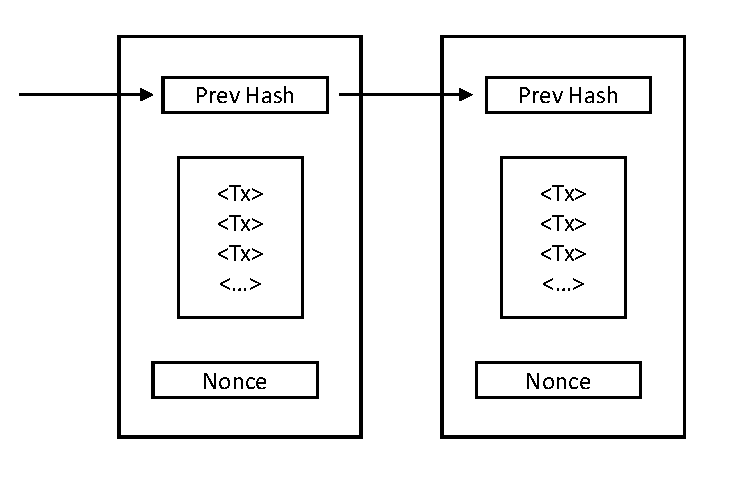
\includegraphics[width=1\linewidth]{images/blockchain_nonce_pdf_cropped}
	\caption{Vereinfachte Darstellung einer Blockchain. \cite{Nakamoto.2009}} 
	\label{fig:Blockchain}
\end{figure}

Da in jedem Block auf das vorherige Element referenziert wird, ist es unmöglich, zu einem späteren Zeitpunkt eine Änderung eine einem Block vorzunehmen oder die Reihenfolge der Blöcke zu ändern. Anzumerken ist, dass die Anforderung an die vorausgehenden Nullen stetig schwanken. Je mehr Nutzer nach Blöcken suchen, desto mehr Nullen werden benötigt. Im Umkehrschluss sinkt bei weniger Minern die Schwierigkeit. Dieses Verfahren wird als \textit{Proof of Work} (POW) bezeichnet.

\subsection{Die 51\%-Attacke als möglicher Angriff auf eine Proof of Work Blockchain}
\label{sec:51attack}
Ein potenzieller Angreifer, nennen wir ihn Mallory, möchte das Netzwerk manipulieren. Die Idee ist es, Bob 1 BTC zu senden, die Transaktion aber nur an Bob zu übertragen und vor den anderen Teilnehmern zu verheimlichen. Folglich hat nur Bob von dem Transfer erfahren und Mallory könnte zu einem späteren Zeitpunkt erneut über die Bitcoin verfügen und anderweitig ausgeben. Nach Absenden der Transaktion an Bob berechnet er eine wie in Abschnitt \eqref{sec:pow_section} dargestellte passende Nonce, sodass die vorangehenden Nullen der vom Netzwerk vorgegebenen Länge entsprechen. Findet Mallory eine passende Nonce, wird der neu erstellte Block an Bob gesendet. Parallel senden alle anderen Teilnehmer des Netzwerks ihre gefundenen  Blöcke an Bob. Da der von M gesendete Block nicht mit den anderen ankommenden Blöcken übereinstimmt, besitzt Bob zwei verschiedene Zustände des Netzwerks: Eine von Mallory manipulierte Version und die korrekte Blockkette. 
\\
Der Konsens besagt, dass in einem solchen Fall nur die längste Blockkette als korrekt anzusehen ist. Damit Bob die von Mallory manipulierte Version der Blockchain nicht verwirft, müsste Mallory konstant neue Blöcke erzeugen. Die Wahrscheinlichkeit, alleine mehr korrekte Blöcke finden zu können als das komplette Netzwerk, ist äußerst gering. Zu einem späteren Zeitpunkt wird Bob den manipulierten Fork des Netzwerks erkennen und verwerfen. Das beschriebene Problem wird als \textit{double-spending problem} bezeichnet. Um einen solchen Angriff auf das Netzwerk erfolgreich ausführen zu können, benötigt der Angreifer mindestens 51\% der Rechenleistung des Netzwerks. \cite{Yang.2019}

\subsection{Bewertung von Proof of Work}
In Abschnitt \eqref{sec:pow_section} wurde das Proof of Work Verfahren vorgestellt. Hinter jedem gefundenen Block steckt enormer Arbeitsaufwand in Form von Rechenleistung. Auf der einen Seite beweist das Finden einer passenden Nonce, dass der Block gültig und die in dem Block niedergeschriebenen Transaktionen ausgeführt wurden. Folglich ist eine spätere Manipulation ausgeschlossen. Auf der anderen Seite verbraucht das Suchen nach neuen Blöcken viel Energie. Je mehr Miner dem Netzwerk beitreten, desto schwieriger wird das Finden neuer Blöcke. Gleichzeitig ist das Netzwerk auf die in einen Block passenden Transaktionen beschränkt. Somit kann das Bitcoinprotokoll und ähnliche Proof of Work Blockchains unabhängig vom Energieverbrauch im Mittel etwa 5 Transaktionen pro Sekunde (TPS) verarbeiten. \cite{Cai.2019}

Über die Jahre hat sich Bitcoin als besonders sicher und dezentral bewiesen. Jeder kann am Netzwerk teilnehmen und die Dezentralität weiter vorantreiben. Dank sicherem POW ist seit Start der Blockchain kein erfolgreicher Angriff bekannt. Der anfallende Rechenaufwand muss in Kauf genommen werden, um das Netzwerk sicher fortführen zu können. 
\section{Blockchaintrilemma}
Das Blockchaintrilemma beschreibt das Vereinen dreier wichtiger Faktoren: Dezentralität, Skalierbarkeit und Sicherheit:

\begin{itemize}
    \item Dezentralisation bedeutet, dass das Netzwerk nicht von einigen Teilnehmern kontrolliert wird. Zusätzlich hat jeder die Möglichkeit, am Netzwerk teilzunehmen
    \item Skalierbarkeit ist die Eigenschaft einer Blockchain, mit steigendem Aufkommen von Transaktionen klarzukommen
    \item Sicher ist eine Blockchain, wenn sie die vorhandenen  Daten vor verschiedenen Attacken schützt
\end{itemize}

Bisherige Blockchainarchitekturen können die drei Punkte nicht vereinen. So ist Bitcoin dezentral und sicher, jedoch unskalierbar. \cite{Abadi.2018} 
\section{Funktionsweise des Chainwebs}
\label{sec:chainweb_overview}
Das Chainweb ist eine öffentlich zugängliche Blockchain. Diese setzt zur Konsensfindung auf das bewährte Proof of Work Verfahren. Die Überlegung ist es, eine POW-Blockchain auf Layer 1 zu skalieren. Das Chainweb besteht aus mehreren unabhängigen und parallelen Ketten. Auf jeder Kette wird ähnlich zu Bitcoin der native Coin KDA geschürft. Zusätzlich wird im Header neben dem vorherigen Block auch auf vorangegangene Blöcke der parallelen Ketten gezeigt. Alle 30 Sekunden wird auf jeder Kette ein neuer Block generiert.  Zur Veranschaulichung dient der in Abbildung \eqref{fig:petersen_graph_10} gezeichnete Petersen-Graph. Die Ordnung des Graphen spiegelt die Anzahl der Ketten wider, der Grad gibt Auskunft über die Anzahl der Kanten eines jeden Knoten und der Durchmesser beschreibt, in wie vielen Schritten maximal ein Weg von Knoten $X$ nach Knoten $Y$ existiert. \cite{Martino.2018} \cite{Martino.2019}

\begin{figure}[h!]
    \usetikzlibrary{graphs,graphs.standard}
    \tikzgraphsset{edges={draw,semithick}, nodes={circle,draw,semithick}}
    \centering
    \tikz \graph[math nodes, clockwise]
        { subgraph I_n [V={0,1,2,3,4}] --
          subgraph C_n [V={5,6,7,8,9},radius=1.25cm];
                    {[cycle] 0,2,4,1,3} };

\caption{Petersen-Graph der Ordnung 10, Grad 3 und Durchmesser 2. \cite{Martino.2018}} 
\label{fig:petersen_graph_10}
\end{figure}

Damit die unabhängigen Ketten untereinander kommunizieren können, wurde das Simple Payment Verification (SPV) entwickelt. Es stellt sicher, dass eine Transaktion von Kette $X$ zu Kette $Y$ gesendet werden kann: \cite{Martino.2018}

\begin{enumerate}
 \item Kette $X$: Nutzer $A$ signiert und sendet Transaktion $T$ der Höhe $H$ an $B$
    \begin{enumerate}[i)]
        \item Prüfen der Signatur
        \item Prüfe $Guthaben(A) >= H$
        \item Löschen von $H$ in $A$ auf Kette $X$
        \item Veröffentlichen der Transaktionsnummer im SPV-Verfahren
    \end{enumerate}
 \item Kette $Y$: Aufrufen von $T$ mit SPV-Verifikation
    \begin{enumerate}[i)]
        \item Prüfen der Gültigkeit der Transaktionsnummer
        \item Auslesen der Transaktion 
        \item Prüfen der einmaligen Nutzung von $T$ auf $Y$
        \item Prüfen, ob Y der vorhandenen Kette entspricht
        \item Prüfen der Gültigkeit des Accounts $B$ auf $Y$
        \item Erstellen von $H$ in $B$ auf $Y$
    \end{enumerate}
\end{enumerate}
Das Verfahren wird so lange angewendet, bis die Transaktion auf der Zielkette angekommen ist. Zur Veranschaulichung soll ein Transfer von Kette 1 auf Kette 7 stattfinden. Dieser läuft unter Berücksichtigung des Petersen-Graph über Kette 6: $1-6-7$.
\\
Somit dauert der Transfer bei Verwendung eines Graphen mit Durchmesser 3 maximal 90 Sekunden.

\subsection{Bestimmung des Durchflusses einer Kette}
\label{sec:durchfluss_kette}
In Abschnitt \eqref{sec:chainweb_overview} wurde die grundlegende Funktion des Chainwebs dargestellt. Jede unabhängige Kette kann im Mittel $M$ Transaktionen pro Sekunde verarbeiten. Um eine Annäherung für $M$ zu finden, wird der in Abbildung \eqref{fig:coin_transfer_example} gezeigte Code verwendet. Es werden mehrere Transaktionen an das Netzwerk auf einer Kette übermittelt, die jeweils einen Transfer eines Tokens beinhalten. Für dieses Beispiel wurde Kette 16 gewählt.

\begin{figure}[h!]
\centering
\setminted{
    xleftmargin=2em,
}
\begin{minted}[
    gobble=4,
    frame=single,
    linenos
  ]{yaml}
    code: "(coin.transfer 'alice' 'bob' 0.001)"
    data:
        alice-keyset:
        keys:
          - 66f952933c308d...6fc16abd5eef
        pred: keys-all
    networkId: mainnet01
    publicMeta:
      chainId: "16"
      sender: "alice"
      gasLimit: 600
      gasPrice: 0.0000001
      ttl: 3000
    keyPairs:
      - public: 66f952933c308d...6fc16abd5eef
        secret: 76943f30f1f3f1...22068782d4fb
        caps: 
          - name: "coin.TRANSFER"
            args: ["alice", "bob", 0.001]
          - name: "coin.GAS"
            args: []
    type: exec
  \end{minted}
    \caption{Senden einer Transaktion in PACT unter Verwendung von YAML.} 
    \label{fig:coin_transfer_example}
\end{figure}

Die Transaktion kann durch den in Abbildung \eqref{fig:bash_yaml} dargestellten Terminalbefehl an das Netzwerk übermittelt werden. Für den Versuch wurde ein BASH-Script geschrieben, welches mehrere hundert Transaktionen pro Sekunde abgesendet.

\begin{figure}[h!]
    \begin{lstlisting}[breaklines]
pact -a transfer.yaml | curl -H 'Content-Type: application/json' -d @- https://api.chainweb.com/chainweb/0.0/mainnet01/chain/16/pact/api/v1/send
    \end{lstlisting}
    \caption{Befehl zum Absenden einer Transaktion durch Aufrufen der transfer.yaml Datei.}
    \label{fig:bash_yaml}
\end{figure}

Das Ergebnis wird in Abbildung \eqref{fig:explorer_chain16_result} dargestellt. Es fällt auf, dass in jeden Block maximal 259 Transaktionen passen. Da das Chainweb alle 30 Sekunden einen neuen Block erstellt und angenommen werden kann, dass alle Ketten den gleichen Durchfluss besitzen, werden pro Sekunde $259 \div 30  \approx 8,6$ TPS verarbeitet. Als Annäherung des Durchflusses auf einer Kette dient $TPS_1 = 8$.

\begin{figure}[h!]
	\centering
	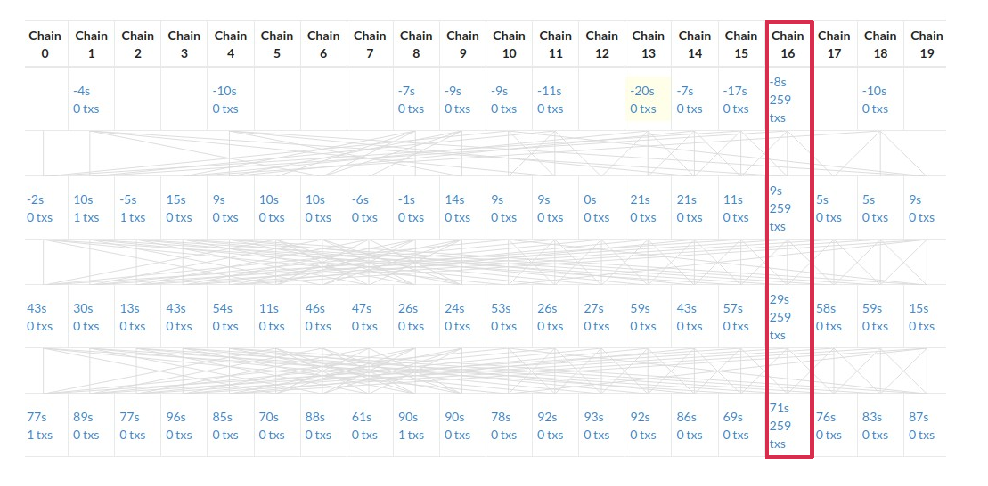
\includegraphics[width=1\linewidth]{images/explorer_crop.pdf}
	\caption{Visuelle Darstellung der Ketten. \cite{KadenaLCC.}} 
	\label{fig:explorer_chain16_result}
\end{figure}

\subsection{Bestimmung des Durchflusses mehrerer Ketten}
Bei dem im Kapitel \eqref{sec:durchfluss_kette} dargestellten Versuch wurde eine Kette verwendet. Doch das Chainweb besteht aus beliebig vielen Ketten $C$. Folglich kann die Anzahl der Transaktionen pro Sekunde durch $TPS_C = C \cdot M$ berechnet werden. Grafik \eqref{fig:tps_chain} stellt den Sachverhalt visuell dar.

\begin{figure}[h!]
    \begin{tikzpicture}
      \begin{axis}[ 
        xlabel=$Ketten \ C$,
        ylabel={$TPS$}
      ] 
        \addplot[domain=0:5000] {x*8}; 
      \end{axis}
    \end{tikzpicture}
\caption{Darstellung des Durchflusses in Abhängigkeit der Ketten.}
\label{fig:tps_chain}
\end{figure}

Man kann erkennen, dass der Durchfluss beim Hinzufügen neuer Ketten linear steigt.

\subsection{Skalierung einer POW-Blockchain durch das Chainweb}
Nun stellt sich die Frage, ob es ein Limit für die Anzahl der Ketten $C$ gibt. Ausschlaggebend dafür sind Grad und Durchmesser des Graphen. In Abbildung \eqref{fig:petersen_graph_10} wurde ein Graph dritten Grades mit dem Durchmesser 2 vorgestellt. Tabelle \eqref{tab:graphentheory} zeigt die mögliche Ordnung eines bekannten Graphen in Abhängigkeit seines Durchmessers $k$ und Grades $d$. 
Es fällt auf, dass mit steigendem Durchmesser und höherem Grad die Ordnung des Graphen steigt. Unter Berücksichtigung der Blockzeit von 30 Sekunden ist ein geringer Durchmesser wünschenswert, da das in Kapitel \eqref{sec:chainweb_overview} beschriebene Simple Payment Verification Protokoll pro Kette eine Blockzeit zur Verifikation benötigt.

Mit $k = 7$ und $d = 7$ wird eine Ordnung von 52 768 erreicht. Übertragen auf das Chainweb entspricht das mit dem zuvor experimentell bestimmten Durchfluss für eine Kette von $TPS_{1} = 8$ für 52 768 Ketten $TPS_{52768} = 52768 \cdot 8 = 422 144$ Transaktionen pro Sekunde. Dieser Wert ist wesentlich höher als bei klassischen Proof of Work Blockchains.

% https://tex.stackexchange.com/questions/89166/centering-in-tabularx-and-x-columns %
\newcolumntype{Y}{>{\centering\arraybackslash}X}
\begin{table*}[t] % top
    \begin{tabularx}{\textwidth}{|c|c|c|c|c|Y|Y|Y|Y|Y|Y|Y|}
        \hline
        \diagbox{d}{k} & 2 & 3 & 4 & 5 & 6 & 7 & 8 & 9 & 10 \\
        \hline
        3 & 10 & 20 & 38 & 70 & 132 & 196 & 360 & 600 & 1 250 \\
        \hline
        4 & 15 & 41 & 98 & 364 & 740 & 1 320 & 3 243 & 7 575 & 17 703 \\
        \hline
        5 & 24 & 72 & 212 & 624 & 2 772 & 5 516 & 17 030 & 57 840 & 187 056 \\
        \hline
        6 & 32 & 111 & 390 & 1 404 & 7 917 & 19 383 & 76 461 & 331 387 & 1 253 615 \\
        \hline
        7 & 50 & 168 & 672 & 2 756 & 11 988 & 52 768 & 249 660 & 1 223 050 & 6 007 230 \\
        \hline
        8 & 57 & 253 & 1 100 & 5 060 & 39 672 & 12 127 & 734 820 & 4 243 100 & 24 897 161 \\
        \hline
        9 & 74 & 585 & 1 550 & 8 268 & 75 893 & 279 616 & 1 697 688 & 12 123 288 & 65 866 350 \\
        \hline
        10 & 91 & 650 & 2 286 & 13 140 & 134 690 & 583 083 & 4 293 452 & 27 997 102 & 600 380 000 \\
        \hline
        11 & 104 & 715 & 3 200 & 19 500 & 156 864 & 1 001 268 & 7 442 328 & 72 933 102 & 600 380 000 \\
        \hline
        12 & 133 & 786 & 4 680 & 29 470 & 359 772 & 1 999 500 & 15 924 326 & 158 158 875 & 1 506 252 500 \\
        \hline
        13 & 162 & 851 & 6 560 & 40 260 & 531 440 & 3 322 080 & 29 927 790 & 249 155 760 & 3 077 200 700 \\
        \hline
        14 & 183 & 916 & 8 200 & 578 37 & 816 294 & 6 200 460 & 55 913 932 & 600 123 780 & 7 041 746 081 \\
        \hline
        15 & 187 & 1 215 & 11 712 & 76 518 & 1 417 248 & 8 599 986 & 90 001 236 & 1 171 998 164 & 10 012 349 898 \\
        \hline
        16 & 200 & 1 600 & 14 640 & 132 496 & 1 771 560 & 14 882 658 & 140 559 416 & 2 025 125 476 & 12 951 451 931 \\
        \hline
    \end{tabularx}
\caption{Ordnung eines Graphen mit Grad $d$ und Durchmesser $k$. \cite{Beardsley.2021}}
\label{tab:graphentheory}
\end{table*}
\section{Hat das Chainweb das Blockchaintrilemma gelöst?}
\subsection{Dezentralität}
Das Chainweb setzt auf Proof of Work. Es erlaubt jedem, ohne Einschränkungen am Netzwerk teilzuhaben. Da Miner oftmals in sogenannten Mining-Pools gemeinsam rechnen, könnte ein koordinierter Angriff auf einen solchen Pool zu einem erfolgreichen 51\%-Angriff führen. Die praktische Durchführbarkeit hängt von verschiedenen Faktoren ab. Es können sich verschiedene Pools zusammenschließen und so einen Großteil des Netzwerks kontrollieren. Abbildung \eqref{fig:chainweb_miner} vermittelt einen Eindruck über die Verteilung der Rechenleistung im Chainweb.

\begin{figure}[h!]
    \centering
    \togglefalse{showpct}
    \begin{tikzpicture}
    \tikzset{lines/.style={draw=white},}
    \pie[color = {cyan, red, blue!80, yellow, green, purple!80},
        sum=auto, 
        after number=,
        text=legend,
        style={lines}]
    {68.03/Poolflare,17.36/Dxpool,5.01/f2pool,2.34/Poolmars,2.11/Kelepool,5.14/Unbekannt}
    \end{tikzpicture}
    \caption{Verteilung der Hashrate des Chainwebs auf Mining-Pools im Juni 2022. \cite{KadenaLCC.} \cite{Anedak.}}
    \label{fig:chainweb_miner}
\end{figure}

Ein Mining-Pool besitzt weit mehr als die Hälfte der Rechenleistung. Würde der Betreiber des Pools böse Absichten entwickeln oder der Pool übernommen werden, könnte ein Angreifer das Netzwerk manipulieren. Der Punkt Dezentralität ist nur eingeschränkt erfüllt. Theoretisch könnte das Chainweb diesen Aspekt vollumfänglich erfüllen, jedoch ist damit für die Miner ein höherer Arbeitsaufwand verbunden, welcher augenscheinlich gescheut wird. Das Rechnen in einem Pool ist unkompliziert und mit geringeren Kosten verbunden. Für den Miner mag das gut sein, für das Netzwerk bedeutet das jedoch mehr Zentralisation.

\subsection{Sicherheit}
Um neue Blöcke zu generieren, wird die Hashfunktion $Blake2S\_256$ eingesetzt. Diese wurde nach dem in Kapitel \eqref{sec:pow_section} vorgestelltem Prinzip implementiert. BLAKE gilt als sehr sichere und effiziente Hashfunktion. Bei BLAKE2 handelt es sich um eine verbesserte Version von BLAKE. Sie wird unter anderem im Linux Kernel und bei OpenSSL eingesetzt. \cite{Espitau.2015} \cite{Blake2.2017}

Weiter wird in jedem Block nicht nur auf den vorherigen Block einer Kette gezeigt. Zusätzlich zeigt jeder neu erstellte Block auch auf die Nachbarketten. Resultierend müsste ein potenzieller Angreifer für einen erfolgreichen 51\%-Angriff auch die parallel laufenden Ketten dominieren. Ein mögliches Szenario bei einer klassischen POW-Blockchain wurde in \eqref{sec:51attack} aufgezeigt. Der Angriff kann auch auf das Chainweb ausgeführt werden. Da jeder Block neben dem Vorgänger auf seiner Kette auch auf Nachbarketten referenziert, muss ein Angreifer deutlich mehr Aufwand betreiben:

Sei $p$ die  Wahrscheinlichkeit, dass das Netzwerk einen neuen Block findet und $q$ die Wahrscheinlichkeit, dass der Angreifer einen neuen Block findet.\\
$q_{\mu(z)}$ entspricht der Wahrscheinlichkeit für den Angreifer $\mu(z)$ Blöcke aufzuholen. Der Angreifer wäre also $z$ Blöcke hinter dem aktuellen Stand des Netzwerks. Der Sachverhalt wird in \eqref{equ:wahrscheinlichkeit_pq} dargestellt.

\begin{equation}
  q_{\mu(z)} =
   \begin{cases}
    1 & \text{$p \leq q$}\\
    (q/p)^{\mu(z)} & \text{$p > q$}\\
    \end{cases}   
\label{equ:wahrscheinlichkeit_pq}
\end{equation}
\\
Der Fortschritt des Angreifers kann durch Gleichung \eqref{equ:angreifer_fortschritt} mittels einer Poisson-Verteilung berechnet werden.
\begin{equation}
    \lambda = \frac{q}{p}\mu(z)
\label{equ:angreifer_fortschritt}
\end{equation}
\\
Um die Wahrscheinlichkeit zu berechnen, dass der Angreifer $z$ Blöcke aufholt, wird Formel \eqref{equ:angreifer_aufholen} verwendet.
\begin{equation}
    \sum_{b=0}^{\mu(z)} \frac{\lambda^{b}e^{-\lambda}}{b!} \cdot \left(\frac{q}{p}\right)^{\mu(z)-b}
\label{equ:angreifer_aufholen}
\end{equation}
Es zeigt sich, dass ein Angreifer über mehrere Blöcke betrachtet keinen Erfolg haben wird. \cite{Martino.2018} \cite{Martino.2018b}
\\
Durch Verwendung einer sicheren Hashfunktion und zusätzliches Referieren auf verschiedene Blöcke gewährt das Chainweb Sicherheit. Zusätzlich setzt es auf Proof of Work, welches richtig eingesetzt als sehr sicher angesehen wird. \cite{Gervais.2016}


\subsection{Skalierbarkeit}
Nach dem experimentellen Bestimmen des Durchflusses in Abschnitt \eqref{sec:durchfluss_kette} und anschließender Übertragung auf mehrere Ketten $C$ wurde gezeigt, dass ein enorm hoher Durchfluss erreicht werden kann. Sobald der mögliche Durchfluss nicht ausreicht, kann durch das Hinzufügen neuer Ketten dieser erhöht werden. Es gibt kein Limit für die Anzahl an Ketten, solange ein passender Graph gefunden werden kann. Mögliche Zusammensetzungen sehr großer Graphen zeigt Tabelle \eqref{tab:graphentheory}. Es kann angenommen werden, dass für den in der Realität benötigten Durchfluss immer ein passender Graph mit möglichst geringem Durchmesser gefunden werden kann. \cite{Loz.2010}
\section{Abschließende Einschätzung}
In dieser Arbeit wurden das Chainweb hinsichtlich dreier Faktoren untersucht. Es wurde gezeigt, wie eine Proof of Work Blockchain auf Layer 1 skalieren kann. Folglich kann das Netzwerk alle aufkommenden Transaktionen verarbeiten. Aktuell besitzt ein Mining-Pool zu viel Rechenleistung, weshalb die Dezentralität nur eingeschränkt gegeben ist. Dies spricht zum einen gegen den Aspekt der Dezentralität. Darüber hinaus resultiert daraus aber auch ein Defizit bei der Sicherheit der Blockchain. Die junge Technologie muss sich erst noch beweisen. Im Blockchainsektor kommen neue Projekte und Technologie genauso schnell, wie diese auch wieder verschwinden. Ob der Ansatz, mehrere unabhängige Ketten zu verwenden, sich schlussendlich als praxistauglich erweist, bleibt abzuwarten.
\section{Literatur}
\printbibliography[heading=none]
\end{document}
